%!TEX root=../master.tex
\chapter{Attack Techniques}\label{attack_techniques}

In order to examine how a smart meter can be abused we need some basic security concepts.
The attacks presented here will relate to the attack trees presented in the previous chapter.
First we will go over cryptography concepts and afterwards a selection of relevant attacks will be explained.

\section{Terms}
Alice and Bob are used to present two parties.
Generally Alice wants to send Bob a secret message.
Eve is used as a third party which is eavesdropping on the communication between Alice and Bob.
This typical setup can be seen on \cref{alice_bob_eve}.

\begin{figure}[H]
  \begin{center}
    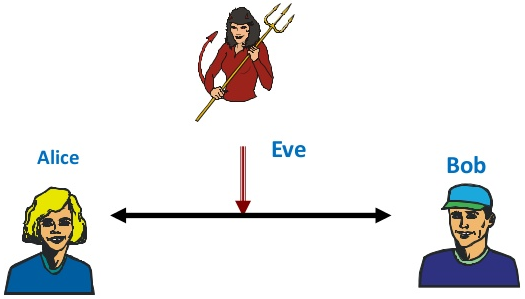
\includegraphics[width=.7\textwidth]{alice_bob_eve}
  \end{center}
  \caption[wat]{Alice, Bob and Eve.\footnotemark}
  \label{alice_bob_eve}
\end{figure}
\footnotetext{\url{https://image.slidesharecdn.com/quantumcryptography-130913005611-phpapp01/95/quantum-cryptography-13-638.jpg?cb=1379033822}}
